\documentclass[a4paper,twoside,phd]{BYUPhys}
% The BYUPhys class is for producing theses and dissertations
% in the BYU Department of Physics and Astronomy.  You can supply
% the following optional arguments in the square brackets to
% specify the thesis type:
%
%   senior  : Produces the senior thesis preliminary pages (default)
%   honors  : Produces the honors thesis preliminary pages
%   masters : Produces the masters thesis preliminary pages
%   phd     : Produces the PhD dissertation preliminary pages
%
% The default format is appropriate for printing, with blank pages
% inserted after the preliminary pages in twoside mode so you can
% send it directly to a two-sided printer. However, for ETD
% submission the blank pages need to be removed from the final output.
% The following option does this for you:
%
%   etd     : Produces a copy with no blank pages in the preliminary section.
%             Remove this option to produce a version with blank pages inserted
%             for easy double sided printing.
%
% The rest of the class options are the same as the regular book class.
% A few to remember:
%
%   oneside : Produces single sided print layout (recommended for theses less than 50 pages)
%   twoside : Produces double sided print layout (the default if you remove oneside)
%
% The BYUPhys class provides the following macros:
%
%   \makepreliminarypages : Makes the preliminary pages
%   \clearemptydoublepage : same as \cleardoublepage but doesn't put page numbers
%                           on blank intervening pages
%   \singlespace          : switch to single spaced lines
%   \doublespace          : switch to double spaced lines
%
% --------------------------- Load Packages ---------------------------------

% The graphicx package allows the inclusion of figures.  Plain LaTeX and
% pdfLaTeX handle graphics differently. The following code checks which one
% you are compiling with, and switches the graphicx package options accordingly.
\usepackage{ifpdf}
\ifpdf
  \usepackage[pdftex]{graphicx}
\else
  \usepackage[dvips]{graphicx}
\fi

%%%%%%%%%%%%%%%%%%%%%%%%%%%%%%%%%%%%%%%%%%%%%%%%%%%%%%%%%%%%%%%%%%
% Edited : Beeshanga
%
% If you need to include any code in the text use this package
% \usepackage{listings}
% It can be used to make key words bold, add colours, etc. Refer
% to http://en.wikibooks.org/wiki/LaTeX/Packages/Listings for
% more information.
%
% For theorems, propositions, proofs and assumtions use this
% package
% \usepackage{amsthm}
% For more information refer to the following website
% http://en.wikibooks.org/wiki/LaTeX/Theorems
%
%%%%%%%%%%%%%%%%%%%%%%%%%%%%%%%%%%%%%%%%%%%%%%%%%%%%%%%%%%%%%%%%%%

% The fancyhdr package allows you to easily customize the page header.
% The settings below produce a nice, well separated header.
\usepackage{fancyhdr}
  \fancyhead{}
  \fancyhead[LO]{\slshape \rightmark}
  \fancyhead[RO,LE]{\textbf{\thepage}}
  \fancyhead[RE]{\slshape \leftmark}
  \fancyfoot{}
  \pagestyle{fancy}
  \renewcommand{\chaptermark}[1]{\markboth{\chaptername \ \thechapter. #1}{}}
  \renewcommand{\sectionmark}[1]{\markright{\thesection \ #1}}


% The cite package cleans up the way citations are handled.  For example, it
% changes the citation [1,2,3,6,7,8,9,10,11] into [1-3,6-11].  If your advisor
% wants superscript citations, use the overcite package instead of the cite package.
\usepackage{cite}

% The makeidx package makes your index for you.  To make an index entry,
% go to the place in the book that should be referenced and type
%  \index{key}
% An index entry labeled "key" (or whatever you type) will then
% be included and point to the correct page.
%\usepackage{makeidx}
%\makeindex

% The url package allows for the nice typesetting of URLs.  Since URLs are often
% long with no spaces, they mess up line wrapping.  The command \url{http://www.physics.byu.edu}
% allows LaTeX to break the url across lines at appropriate places: e.g. http://www.
% physics.byu.edu.  This is helpful if you reference web pages.
\usepackage{url}
\urlstyle{rm}

% If you have a lot of equations, you might be interested in the amstex package.
% It defines a number of environments and macros that are helpful for mathematics.
% We don't do much math in this example, so we haven't used amstex here.
\usepackage{amsmath}
\usepackage{amssymb}
\usepackage{subfigure}
\usepackage{cite}
\usepackage{amsxtra}
\usepackage{amsfonts}
\usepackage{graphicx}
\usepackage{multirow} % This is package for multi-rows in tables added on 7th July 2009 by Arif
%\usepackage{setspace}

% The caption package allows us to change the formatting of figure captions.
% The commands here change to the suggested caption format: single spaced and a bold tag
\usepackage[labelfont=bf,labelsep=colon]{caption}%[2008/04/01]
 \DeclareCaptionFormat{suggested}{\singlespace#1#2#3\par\doublespace}
 \captionsetup{format=suggested}


\usepackage{array}
\usepackage{multirow}
\usepackage{verbatim}
\usepackage{enumerate}

% Defining the symbols




% The hyperref package provides automatic linking and bookmarking for the table
% of contents, index, equation references, and figure references.  It must be
% included for the BYU Physics class to make a properly functioning electronic
% thesis.  It should be the last package loaded if possible.
%
% To include a link in your pdf use \href{URL}{Text to be displayed}.  If your
% display text is the URL, you probably should use the \url{} command discussed
% above.
%
% To add a bookmark in the pdf you can use \pdfbookmark.  You can look up its usage
% in the hyperref package documentation
\usepackage[bookmarksnumbered,pdfpagelabels=true,plainpages=false,colorlinks=true,
            linkcolor=black,citecolor=red,urlcolor=blue]{hyperref}

% ------------------------- Fill in these fields for the preliminary pages ----------------------------
%
% For Senior and honors this is the year and month that you submit the thesis
% For Masters and PhD, this is your graduation date
  \Year{2018}
  \Month{November 09,}
  \Author{Abhishek Satpathy}

% If you have a long title, split it between two lines. The \TitleBottom field defines the second line
% A two line title should be an "inverted pyramid" with the top line longer than the bottom.
    \TitleTop{Protocol for Smart Contract Communication}
  \TitleBottom{Among Blockchains} % edited Beeshanga
 \DegreeTitle{Bachelor of Engineering
 \\ Software Engineering Stream} % edited Beeshanga

% Your research advisor
 \Advisor{Supervisor: Michael Johnson}

% The department undergraduate research coordinator
%  \UgradCoord{A}

% The representative of the department who will approve your thesis (usually the chair)
%  \DepRep{B}

% Acknowledge those who helped and supported you

  \Acknowledgments{
  \vspace{-1.5cm}
    \noindent I would like to acknowledge my supervisor Prof. Michael Johnson who has always been a great help throughout my degree and not just this thesis. Michael accepted to supervise my project proposal even though it was not related to one of his areas of research. 
    
    
    \noindent I would also like to acknowledge Mr. Kris Crnomarkovic who has been really helpful with long and tiring discussions about certain difficult issues that I encountered during research. Kris's involvement with my theses is really appreciated.

  }


% The title of the department representative
%  \DepRepTitle{Chair}
  \Statement{
    \noindent I, Abhishek Satpathy, declare that this report, submitted as part of the requirement for the award of Bachelor of Engineering in the School of Engineering, Macquarie University, is entirely my own work unless otherwise referenced or acknowledged. This document has not been submitted for qualification or assessment at any other academic institution.
    \vspace{0.5cm}

    \noindent     Student's Name: Abhishek Satpathy

    \vspace{0.25cm}

    \noindent Student's Signature: Abhishek Satpathy

    \vspace{0.25cm}

    \noindent     Date: \today
    }

% The text of your abstract
\Abstract{
\vspace{-1.5 cm}
Blockchain technology has potential applicability in finance, supply-chain management, asset-tracking, web decentralization. Scalability and interoperbility are two major problems, hindering the applicability of blockchains in large-scale commercial architectures. Here, we discuss the application of a novel protocol that aims to solve the issues of scalability and interoperability of blockchains using a communication layer between multiple homogenous blockchains.
}



% Statement of Candidate



\fussy

\begin{document}

 % Start page counting in roman numerals
 \frontmatter

 %This command makes the formal preliminary pages.
 % You can comment it out during the drafting process if you want to save paper.

 \makepreliminarypages


%\clearemptydoublepage
\doublespace
%\include{Publications/publications}

% \clearemptydoublepage
%\include{Organization/organization}

 \clearemptydoublepage
\singlespace
 % Make the table of contents.
 \tableofcontents

\clearemptydoublepage
% Make the list of figures
\listoffigures

\clearemptydoublepage
% Make the list of tables
\listoftables

\clearemptydoublepage

% Start regular page counting at page 1
\mainmatter
%
\chapter{Introduction}
\label{chap:Introduction}
Blockchain technology has demonstrated enormous potential utility in multiple fields including "Internet of things", governance, finance, asset-tracking and web decentralization. However, the adoption and use of blockchains into production grade systems is yet to be demonstrated. 
 Scalability and inter-operability are major problems, hindering the production grade adoption of blockchains into these different fields of application. Blockchain systems currently are crippled by extremely low transaction  throughput which makes their use impractical in real world use cases. Available blockchain implementations are practically limited to around 30 transactions per second. This issue of limited transaction throughput arises from the current synchronous consensus mechanisms which require a wide time margin to ensure safety of the transactions. The demand for higher transaction throughput is rapidly increasing with the growing user base. One of the  ways of addressing this scalability problem is facilitating intercommunication among smart contracts on multiple separate blockchains. This intercommunication protocol inherently solves the problem of inter-operability along with scalability. In this thesis we lay out the design and implementations specifications of such a protocol that facilitates the inter-operability of multiple compatible blockchains.

\section{Project Goal}
The goal of this project is to lay out the design, implementation and testing specifications of a layer two blockchain solution that facilitates high transaction throughput and inter-operability among multiple blockchain systems. Layer two, here, is defined as a system that is built on top of a layer one blockchain system like ethereum or bitcoin and therefore relies on the layer one chain for security. Layer two solutions are built without requiring any breakthrough modifications to the existing layer one architecture. The project is specifically going to focus on a protocol that is built on top of ethereum as the foundation layer one blockchain. The biggest challenge for the implementation of this project is ensuring that the layer two solution is at least as secure as the existing foundation that it is built upon. The protocol has to balance between keeping a high transaction throughput and maintaining a high level of decentralization. Decentralization and transaction throughput can easily get inversely intertwined in a decentralized system architecture and therefore precaution needs to be taken while designing the system to reduce centralization.
\\
\\ One of the other goals of the project will also be to lay out the modifications to the existing foundation system that would allow the integration of the layer two system to the foundation architecture. The project does not aim to create a completely new blockchain architecture.
\section{Project Planning}
The project planning was done over the last six months during the course of ENGG 460. There have been a lot of changes the initial plan that was developed during ENGG 460. The biggest change however has been to the scope, deliverables and timeline of the project. These changes are discussed below in their respective sections.

\subsection{Scope}
The project scope has remained very similar to the scope that was described in the initial project plan. The scope is to deliver a protocol for intercommunication and interoperability of smart contracts. The scope in the initial project plan might have indicated that the scope includes the delivery of a prototype of such a blockchain architecture; however, the new scope of the project includes only the system requirements, design and testing specifications of the protocol. 
\subsection{Deliverables}
In the initial plan the project had two deliverables. One of the deliverables for the project was a suite of smart contracts on different ethereum blockchains such that those smart contracts can send messages and transactions among themselves. The other deliverable in the initial protect plan was a react-native app that would be able to demonstrate the functionality of the smart contracts. There has been a change in the deliverables for the project over the course of the last six weeks of progressing through the development. 
\\

The new deliverable for the project is a protocol for intercommunication and the interoperability of multiple blockchains. The deliverable includes system requirements, system design and testing specifications. However, any working prototype of the protocol is not a hard deliverable of the project.
\subsection{Timeline}
There have been significant changes to the timeline of the project as it has progressed over the last six weeks. The reason for these changes is the change in the deliverables for the project. The deadline for the project was assumed to mid December in the previous project plan; the new deadline is 9th of November which is a hard deadline. Moreover, a lot of variables and deliverables had unknown components with estimated timeframes. The timeline has a become firmer with most of the variables becoming clearer. The new GANTT chart with the updated timeline for the project is shown below.
\section{Project Background}
Prior to starting in on blockchain systems, one needs to be familiar with supporting technologies that support and facilitate the working of blockchains. 
\subsection{Cryptographic Hash Function}
A cryptographic hash function is a one way mathematical construct that takes a data input of arbitrary length and outputs arbitrary data of a fixed length. The primary use of hashing in cryptography is maintaining the integrity of messages. Hashes are used in a blockchain to ensure the integrity of the data stored in each block. The data or the list of transactions in a block is hashed and the hash is appended to the next block, this ensures the integrity of the data because if even a single bit of the data is manipulated then the new hash of the block is completely different. The hash function used in the protocol described in this paper is Keccac-512 which is a variation of the SHA-512 hashing algorithm. 
\subsection{Public Key Cryptography}
Public Key Cryptography is one of the core technologies used in a blockchain system. The accounts on a blockchain are a hashed version of the public key of the user. The accounts can be accessed 
\subsection{Consensus}
Consensus is a mechanism which ensures that every node on the blockchain network has the same exact copy of the data. A consensus mechanism syncs data across all nodes as and when those nodes connect to the network. Consensus also works as a fault tolerance mechanism which is essential in any distributed computing setup suck as a distributed ledger to avoid corrupt nodes. Proof of work is by far the most popular consensus mechanism used in mainstream public blockchains. It is a ultimately a variation of the popular Practical Byzantine Fault tolerance algorithm.
\subsection{State Transition Machine}
The state on a blockchain is a mapping between the account addresses and the state of the account in terms of the transaction history. Every transaction on the blockchain is a manupulation of the state. The blockchain itself acts as a state transition machine which facilitates transactions by allowing the valid ones to manipulate the state.
\subsection{Clients}
A client of the blockchain is the end-user software that ensures the blockchain synchronisation, generates and stores private keys, and facilitates transactions on behalf of the private key. Clients live on user hardware which act as an interface between the user's device and the blockchain network.
\subsection{Transactions}
A transaction is a the transfer of a signed data package on the blockchain which manipulates the state of the ledger. It is a record of a valid computational activity that has taken place. Any information that is stored and can be retrieved is the result of a transaction. EVM transactions involve transfer of value as the transaction themselves have a cost attached to them. 
\subsection{Smart Contracts}
Smart Contracts are agents that facilitate the negotiation of a transaction on the blockchain without the use of another third party agent. Smart contracts are the only entry point to the state of the blockchain and therefore the only party that can modify the data layer on the ledger.

\chapter{Background and Related Work}
Before any meaningful research is done on the topic, it is quite essential to review the available literature on the topic. The process of reviewing existing literature review helps one to understand the cutting edge research on the topic and also familiarize oneself with failures and successes. This chapter reviews the existing literature and work done in the area of increasing blockchain transaction throughput by facilitating interoperability of blockchains. The most important thing to note is that there is a serious lack of quality academic literature in the field as the research in the field is quite new and hasn't percolated into academia yet. Therefore, most of the available literature is from research work done by blockchain startups and the available whitepapers. The language in those whitepapers is often not very academic and therefore one of the most important tasks in this chapter would be to interpret the whitepapers critically and translate the language into proper academic form.
\section{Ethereum}
The entire framework of this project is based on the ethereum protocol. Therefore, the discussion on ethereum is unavoidable. Ethereum is a decentralised value transfer system made possible using a cryptographically secure, transaction-based state machine. A blockchain or a distributed ledger in simple terms. Ethereum was first developed by Vitalik Buterin in late november 2013. It was a complete rewrite of the bitcoin system with addition of a turing-complete virtual machine and smart contract execution capability. In ethereum's state transition machine, the final state also referred to as the canonical state is a result of a consensus mechanism using a simplified version of the GHOST protocol.

\subsection{Blocks, State and Transactions}
\subsubsection{Blocks}
The block in Ethereum is a collection of transaction bunched together as a set. The block has three parts, a block header, the transactions, and the ommers which is a collection of related block headers. The block header contains the following pieces of information:
\begin{description}
\item[$\bullet$ parentHash:] a Keccak 256-bit hash of the previous block's header
\item[$\bullet$ ommersHash:] a Keccak 256-bit hash of the ommers list or the list of blocks which have the same parent block as the current block
\item[$\bullet$ beneficiary:] the 160-bit address of the account to which all the gas fee has to be transferred
\item[$\bullet$ stateRoot:] a Keccak 256-bit hash of the root node of the state trie
\item[$\bullet$ transactionsRoot:] a Keccak 256-bit hash of the root node of the trie containing all the transactions in the current block
\item[$\bullet$ receiptsRoot:] a Keccak 256-bit hash of the trie containing the reciepts of all the transactions in the current block
\item[$\bullet$ logsBloom:] bloom filter composed of index-able log entries for transaction receipts
\item[$\bullet$ difficulty:] a number corresponding to the difficulty level of the block
\item[$\bullet$ number:] a scalar value corresponding to the number of ancestor blocks of the current block. The genesis block does not have an ancestor block and hence, it is conventionally assigned a number 0.
\item[$\bullet$ gasLimit:] a scalar value equal to the maximum limit of gas expenditure of the block
\item[$\bullet$ gasUsed:] a scalar value equal to the total gas used in transactions in the block
\item[$\bullet$ timeStamp:] a reasonable output of the Unix's time at the block's inception
\item[$\bullet$ extraData:] arbitrary byte array containing block metadata
\item[$\bullet$ mixhash:] a 256-bit hash which together with the nonce proves that a sufficient amount of computation has been carried out on this block
\item[$\bullet$ nonce:] a 64-bit hash which together with the mix-hash proves that a sufficient amount of computation has been done on this block
\end{description}
\subsubsection{World State}
The world state is a mapping between account addresses which are 160 bit hashed versions of the public keys and account states. This mapping is stored in a data-structure called a Merkle Patricia tree. The account states comprise of the following fields;
\begin{description}
\item[$\bullet$ nonce:] it is a value that is equal to the number of transactions sent from the account
\item[$\bullet$ balance:] a value equal to the number of wei owned by the address
\item[$\bullet$ storageRoot:] a 256-bit hash of the root node of the merkle patricia tree that contains the storage data of the account
\item[$\bullet$ codeHash:] the hash of the EVM code of the account, which gets executed in case of transactions
\end{description}
\subsubsection{Transactions}
A transaction is formally a single cryptographically signed instruction executed by an external party. There are two types of transactions in Ethereum: the first type results in a message call between actors and the second type results in creation of new accounts. A transaction primarily has the following fields:
\begin{description}
\item[$\bullet$ nonce:] a value equal to the number of transactions sent by the sender
\item[$\bullet$ gasPrice:] number of wei to be paid for each unit of gas. Gas is a computational unit in the EVM which is discussed in a later section.
\item[$\bullet$ gasLimit:] maximum amount of gas that should be utilised for executing this transaction
\item[$\bullet$ to:] a 160-bit address of the message call's recipient 
\item[$\bullet$ value:] number of wei to be transferred to the message call's recipient
\end{description}
A contract creation account contains the following additional fields:
\begin{description}
\item[$\bullet$ nonce:] infinite size byte array containing the EVM code for account initialisation
\item[$\bullet$ data:] infinite size byte array containing the input data of the message call
\end{description}
\begin{description}
\item[]
\end{description}
\subsection{Gas and Transaction Execution}
Gas and transactions are the core of the ethereum computation engine. Transactions forms the basis for all the computation and Gas forms the basis of all payment calculation in ethereum.
\subsubsection{Gas}
Gas is defined as any programmable computation in ethereum. The Ethereum Virtual Machine is a turing-complete computation engine and it is absolutely essential to limit the possibility of denial-of-service attacks in a public computation engine. Gas costs ether to execute and therefore prevents denial-of-service as no ethereum account is likely to have an infinite amount of ether. Every transaction has a gas price which is the amount of ether paid per gas or computational step. Miners will usually preferably select a transaction which has the highest gas price.
\subsubsection{Sub-state}
A valid transaction in ethereum is defined as a transaction which:
\begin{description}
\item [$\bullet$ is a well formed RLP;]
\item [$\bullet$ has a valid signature;]
\item [$\bullet$ has a valid nonce;]
\item [$\bullet$ has a gas limit which is not less than the intrinsic gas;]
\item [$\bullet$ has a sender whose account balance greater than the gas cost]
\end{description}

A transaction is also the most complex part of the ethereum virtual machine as it involves the state transition mechanism. The virtual machine gets in transition state during the execution of the transaction, called the substate. The substate creates a set of temporary accounts needed to complete the transaction, called the suicide set.

The ethereum state transition function is defined as follows: \[\sigma' = \upsilon(\sigma, T)\]
where $\sigma$ is the state and $\Upsilon$ is the state transition function.

\subsection{Canonicalisation}

\subsection{Message Call}

\section{Polkadot}
Polkadot is another approach by the ethereum community to solve the issue of scalability and interoperability by developing a multi-chain framework. Currently, Polkadot is far from being a working system or a prototype 
\section{Cosmos}
Cosmos is a platform which facilitates the interoperability of multiple parallel blockchains while retaining the inherent security features of blockchains. One of the problems faced by interoperable multi-chain frameworks is their vulnerability to an attack if a majority of the hashing ability is not merge-mined with the central parent chain. Cosmos addresses this issue by having multiple independent blockchain which are called zones in Cosmos. The central or the parent chain is called the Cosmos hub. The zones utilise something called a Tendermint Core, which is a Practical Byzantine Fault Tolerant consensus engine. The system described in this paper uses Tendermint and it will be discussed in a later section.

The main currency on the Cosmos hub is a multi-asset proof-of-stake token. The hub and zones facilitate the intercommunication between the hub and the zones using a protocol called the interblockchain comunication protocol, which works on a virtual UDP layer for blockchains.

\subsection{Consensus}
Cosmos uses a partially synchronous BFT (Byzantine Fault Tolerant) consensus algorithm called Tendermint. It uses optimal Byzantine Fault Tolerance with a super majority of greater than 2/3 of the total voting power. Hence, greater than a third of the total voting power has to be Byzantine to cause a violation of safety. In case, a violation occurs, it can be detected by the system by detecting conflicting blocks. And since Cosmos combined with Tendermint is a permissioned system, it is much easier to detect Byzantine nodes.

\subsection{The Hub and Zones}
The Hub and different zones in Cosmos are connected using a protocol called Interblockchain-communication (IBC) protocol. The block commits in the zones are are constantly posted on the hub, allowing the hub to keep track of the world state and also the state of the zones. The zones communicate among each other using the IBC protocol, by sending Merkle-proofs of transactions. 
\subsubsection{The Hub}
The Cosmos hub is the central blockchain in the system which hosts a distributed ledger that supports multiple tokens. These coins are moved from one zone to another using a speacial packet in IBC called a coin packet. The hub is accountable for counting the total amount of coins in each hub. The hub is the central ledger responsible for the entire network of the zones and therefore, is a single point of failure. The security of the hub is of paramount importance. It is secured by a global set of validators which are all permissioned nodes.
\subsubsection{The Zones}
The Zones exchange information among each other via the hub using the IBC. A zone is a essentially a multi-asset, multi-signature account. The hub ensures that the zones cannot transfer more tokens than it has been assigned. The hub does not verify the authenticity of the zones and therefore it should within the senders' discretion to send tokens across zones. 
\subsection{Inter-blockchain Communication (IBC)}
The Inter-blockchain communication (IBC) works by moving packets of data from one zone to another via the hub by posting Merkle-proofs. The proof is evidence that the sending chain published a packet which was meant for the receiving chain. 

The IBC is the most important component of the Cosmos literature. IBC is mentioned here because a lot of inspiration for communication between different blockchains, which have been mentioned in later chapters actually come from the IBC protocol. As shown in the diagram below, the IBC has two different types of transactions; namely, IBCBlockCommitTx transaction and an IBCPacketTx transaction. The IBCBlockCommitTx allows a zone to prove to any observer zone that its most recent block hash exists. The IBCPacketTx allows a zone to prove to any observer that a published packet was indeed sent by the sender. The separation of the two different types of transactions allows the sender and receiver zones to have independent control over their block commits, respectively. The IBCBlockCommit interaction diagram which shows the two types of transactions has been shown in figure 2.1 above.
\begin{figure}
  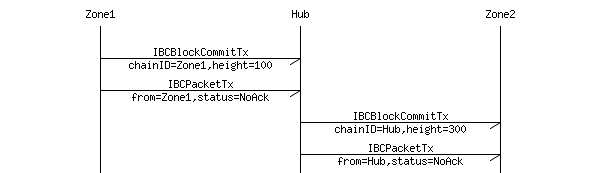
\includegraphics[width=\linewidth]{ibc_transactions.png}
  \caption{IBCBlockCommit Transaction interaction diagram.}
  \label{fig:1}
\end{figure}

\section{Zilliqa}
Zilliqa is another blockchain solution which aims to solve the problem of scalability by using blockchain sharding. It divides the mining network into smaller shards, each capable of processing transactions in parallel. It also has a smart contract execution environment or a virtual machine and a special contract language which implements data-flow programming. This allows the parallel processing of the programs as soon as all the inputs are available. The entire system in Zilliqa is divided into six layers. This layering system is good for maintenance and abstraction of different parts of the system. The layers are explained in more detail in the sections below:

\subsection{Cryptographic Layer}
Zilliqa's cryptographic layer uses elliptic curve cryptography for digital signatures and a memory hard hash function for proof-of-work (PoW). The hash function used in Ziliqa is ethash, which is the hash function used in ethereum. Ethhash is based on Keccak, which is memory hard meaning that Application specific integrated circuits (ASIC) will not be able to generate the hashes. 
\subsubsection{EC-Schnorr Signature}
Zilliqa uses digital signatures based on the EC-Schnorr algorithm instantiated with the secp256k1 elliptic curve. According to Zilliqa, EC-Schnorr has a few benefits over Elliptic Curve Digital Signature Algorithm (ECDSA). Those benefits are Non-malleability, Multisignature ability, and faster speeds. 

\subsubsection{Proof of Work}
Zilliqa uses Proof of Work to prevent Sybil attacks and generate node identities. This is contrary to other blockchain systems such as Ethereum which use PoW for the purpose of achieving consensus. Sybil attacks work by forging identitites of different systems in order to subvert the reputation of the concerned system, especially in used in peer-to-peer networks. Zilliqa uses ethhash as its algorithm of choice for PoW. As mentioned earlier, ethash is a memory hard hash function and requires a considerable amount of memory and high bandwidth I/O interface which makes it impossible to use specialised hardware for computation of the hash.
\subsection{Data Layer}
The data layer mainly consists of the global state of Zilliqa and it also defines the data needed by different entities to update the global state. 
\subsubsection{Accounts and Addresses}
Zilliqa just like ethereum is an account based blockchain system and consists of two types of accounts; namely, a normal account and a contract account. A normal account is created when the EC-Schnorr algorithm is invoked to create a private key. A contract account is created when a contract is deployed by another normal account. The public key is then derived from the private key by using the EC-Schnorr algorithm. The account address for a normal account is then generated by using the 160 least significant bits of the SHA-3 hash of the public key and for a contract account it is generated by using the 160 least significant bits of the SHA-3 hash of the address of the creator's account and the account nonce, which is the number of transactions sent from the particular account. The equations for generating the addresses for both normal and contract accounts are given below:
\begin{equation}
    A_{normal} = LSB_{160}(SHA3-256(PubKey(sk)))
\end{equation}
\begin{equation}
    A_{contract} = LSB_{160}(SHA3-256(address||nonce))
\end{equation}
There are two types of states in Zilliqa; the account state and the global state.
Each account is associated with an account an account state which has the following information:
\begin{description}
\item[$\bullet$ account nonce:] the number of transactions sent from the account in case of a normal account, or the number of transactions sent from the creator's account in case of a contract account.
\item[$\bullet$ balance:] a number that corresponds to the number of tokens currently owned by the respective account.
\item[$\bullet$ code hash:] for a contract account it is the SHA-3 hash of the contract code and for a normal account it is the SHA-3 hash of an empty string.
\item[$\bullet$ storage root:] the SHA3-256 digest of the storage of the account which is a key,value store.
\end{description}
The global state in Zilliqa is the mapping between account addresses and corresponding account states. 
\subsubsection{Transactions}
A transaction in Zilliqa is always sent from a normal account and it updates the global state as it updates the account states of the respective parties involved in the transaction. A transaction contains the following information:
\begin{description}
\item[$\bullet$ version:] current version of the global state.
\item[$\bullet$ nonce:] a number corresponding to the number of transactions sent by the sender's account.
\item[$\bullet$ to:] receiver's account address or in case of a contract creation the rightmost 160 bits of the SHA3-256 hash of an empty string
\item[$\bullet$ amount:] the amount to be transferred in the transaction
\item[$\bullet$ gas price:] the price the sender is willing to pay per Gas for the transaction
\item[$\bullet$ gas limit:] the maximum amount of gas that can be utilised to execute the transaction
\item[$\bullet$ code:] a byte array that contains the contract code in case of a new contract account
\item[$\bullet$ data:] a byte array that specifies the any data needed to process the transaction
\item[$\bullet$ pub key:] the public key of the sender's account that is used to verify the EC-Schnorr signature
\item[$\bullet$ signature:] the EC-Schnorr signature the data package
\end{description}
\subsubsection{Blocks}
Most of the Zilliqa protocol until now has been very similar to ethereum but the diferences actually exist at the block level. There are two types of blocks in Zilliqa which implies two different blockchains, one of which is used for purpose of parallel processing of transactions by multiple shards. The two types of blocks are transaction blocks and directory service blocks (DS-Blocks). The transaction blocks are the normal blocks that would be expected to exist in any blockchain system to keep a record of the transactions. The DS-blocks, however, contain metadata about miners participating in transactions in shards to maintain consensus. The DS-block has two parts; the header and the signature. The header part of the DS-block contains the following data:
\begin{description}
\item[$\bullet$ version]
\item[$\bullet$ previous hash]
\item[$\bullet$ pubkey]
\item[$\bullet$ difficulty]
\item[$\bullet$ number]
\item[$\bullet$ timestamp]
\item[$\bullet$ mix hash]
\item[$\bullet$ nonce]
\end{description}
And the signature part of the DS-block contains only two fields: an EC-Schnorr signature and a bitmap which records a 0 or 1 depending on whether the i-th node participated in the signature.
\\
\\
The transaction blocks, as the name suggests,  keep a record of all the transactions in the blockchain and have three parts; the header, the data, and the signature. The header part consists of the following fields:
\begin{description}
\item[$\bullet$ type:] could be a micro block or a final block.
\item[$\bullet$ version] 
\item[$\bullet$ previous hash]
\item[$\bullet$ gas limit]
\item[$\bullet$ gas used]
\item[$\bullet$ number]
\item[$\bullet$ timestamp]
\item[$\bullet$ state root]
\item[$\bullet$ transaction root]
\item[$\bullet$ tx hashes]
\item[$\bullet$ pubkey]
\item[$\bullet$ pubkey micro blocks:] contains public keys of member who finalised the block. This is present only in final blocks.
\item[$\bullet$ parent block hash]
\item[$\bullet$ parent ds hash]
\item[$\bullet$ parent ds block number]
\end{description}
The data part of the transaction block contains the tx count, which is the number of transactions contained in the block, and the tx list, which is the list of transactions in the block.
\\
\\
Finally, the signature part of the transaction block contains the EC-Schnorr based multi-signature, which contains two field; the signature and the bitmap, that specifies the signatories.  
\\
\\
Micro blocks are submitted by mining shards which then get approved by the DS-commitee to final block status which form a part of the final transaction blockchain.
\subsection{Network Layer}
 Zilliqa's mining network, as mentioned before, is divided into multiple shards which are all capable of processing transactions in parallel. Network sharding is a two step process which involves a dedicated set of special nodes called the Directory Service Committee (DS committee). 
\subsection{Consensus Layer}
The DS committee has to run the consensus protocol on the micro blocks in order to finalise the blocks. Zilliqa uses Practical Byzantine Fault Tolerance (PBFT), however, uses a slightly modified PBFT protocol which includes native multisignatures using EC-Schnorr to improve efficency. Using EC-Schnorr multisignature reduces the communication latency from \[O(n^2)\] to \[O(n)\] and reduces the signature size from O(n) to O(1).
\\
\\
Every consensus round is executed in three rounds:
\begin{description}
\item[$\bullet$] in the pre-prepare phase, the leader of a consensus shard distributes the next transaction micro block.
\item[$\bullet$] in the prepare phase, the nodes validate the block and multicast a message to other nodes
\item[$\bullet$] in the commit phase, after receiving 2/3n commit messages, the group commits the nominated micro block to a final block by performing a second round of EC-Schnorr multisignatures.
\end{description}
\subsection{Smart Contract Layer}
Zilliqa comes with a smart contract execution environment which follows a data-flow programming paradigm. The nodes in Zilliqa's execution model get activated as soon as all the data inputs are available. According to Zilliqa, the advantage of implementing a data flow paradigm is that a lot of nodes can get activated at the same time as soon as all the data points are available. The smart contract language in Zilliqa is not a turing-complete a language, which makes it very application specific. 

\section{Tendermint}

\label{chap:LitReview}

\chapter{System Requirements}
\label{chap:singleuser}

\section{System Overview \label{sec:Intro-ChapUserSelec}}
\subsection{Overall Description}
Blockchain systems have been facing major bottlenecks in the areas of scalability and interoperability. In order for blockchains to be applicable in commercial production-scale applications, the issue of scalability and interoperability need to be solved. This chapter lays out the system requirement specification for a production-grade blockchain system that is scalable and can interoperate with a multitude of other systems.
\subsection{Product Perspective}
The recent hype about blockchain systems has been phenomenal, however, ignoring all the hype, blockchains practically have a lot of applications in many different fields. The system specified in this thesis will have applicability in banking infrastructure, accounting applications, supply chain systems, and digital currencies. Many industry specific applications that require multiple parties to collaborate securely could potentially implement this system in their existing aerchitecture. The system will improve the overall system security, tamper-proofness along with all the other benefits like having continuous history logging that come with any blockchain system.
\subsection{User Characteristics}
The users of the system will mostly be large corporations and conglomerates who have a lot of parties involved in executing a single complete transaction. The product will have three primary classes of users:
\begin{description}
\item[$\bullet$ Primary Users:] Large financial institutions like banks, supply chain management and logistics conglomerates such as DHL and Maersk, and accounting firms like PWC will be the primary uses of the system. The system specified here will remove all the complications such firms have to go through because they have to collaborate with multiple parties in order to process through a single transaction.
\item[$\bullet$ Secondary Users:] The secondary users will be the customers of these large corporations. These users will generally be relying on the large corporations to manage their assets and logistics. These users would have an entry point to the blockchain architecture but they are not the main stakeholders in the system.
\item[$\bullet$ Admin Users:] This class of users are particularly important for the system becasue they have unparalleled access to manage and modify the system. They will all be the top of the level executives of all the corporations involved as parties in the system. These users are allowed to set rules, modify rules, vote on administrative changes and can act as the administrative back-end of the entire system. High level of mutual collaboration and goodwill is expected of them. 
\end{description} 
\subsection{Constraints}
The system defined in the specifications described below has some constraints associated with it. This a result of all the assumptions that were made in the process of designing the system. The design, however, is very modular and all the features designed according to those assumptions can be optimised as per the real-world scenarios during the integration phase.
\\
\\
The following constraints are placed on the system as of the design phase.
\begin{description}
\item[$\bullet$ Legal Constraint:] That the system is financially sound and does so without breaching any financial regulations, both intentionally or unintentionally.
\item[$\bullet$ Safety Constraint:] The system relies on the safety features of existing blockchain architectures and, therefore, the safety of those external systems cannot be guaranteed. However, relying on the safety of other blockchain systems should be a safe bet, as blockchains have a proven track record of safety.
\end{description}
\subsection{Assumptions and Dependencies}
Along with constraints, some assumptions have also been made in the design and specification of the system. The following assumptions have been made in this software requirements specification:
\begin{description}
\item[$\bullet$] The existing systems and infrastructure of the primary users are compatible with the system described here. No compatibility or integration analysis has been done at all.
\item[$\bullet$] The primary users have an existing collaborative and administrative architecture in place which would make it easier for the integration and collaborative use of the system possible and hassle free.
\item[$\bullet$]  The system features laid out in this paper all rely on information obtained from reputed existing systems that are assumed to have been working as described in the resources. Therefore, assumptions have been made about the technical working and compatibility of the system's integration.
\end{description}
\section{System Features \label{sect:chap2sysmodel}}
The following sections in this document intend to describe the important system features of the blockchain interface being described in this paper and provide the interface stimulus/response sequence along with the functional requirements.
\subsection{Token Conversion}
\subsubsection{Description and Priority}
The requirements in this section describe how the system is able to convert between various tokens of different types native to the multiple blockchains connected to the system. The token conversion system is the most important feature of the system as it would facilitate the interoperability of the blockchains operating within the infrastructure. One of the main goals this system intends to achieve is to interoperate among multiple blockchains by transferring tokens among then. Hence, this is a high priority system feature.
\subsubsection{Stimulus/Response Sequence}
The stimulus from different classes of users and response by the system, specific to this system feature is detailed below:
\begin{description}
\item[$\bullet$ Primary Users:] Stimulus: Initiate an intercontinental financial transaction such as money transfer.
\\
\\
Response: The token conversion happens in the central blockchain of the architecture and , funds are transferred, and both parties get a receipt of the transaction.
\item[$\bullet$ Secondary Users:]
Stimulus: Log in to the system's, user facing interface and check the ownership of their funds and assets.
\\
\\
Response: The system logs the user in correctly using the private keys stored in their device and displays a record of their funds and assets.
\item[$\bullet$ Admin Users:] Stimulus: Manage token conversion policies and put up and vote on token conversion policy proposals, that they intend to implement by getting enough votes on their proposal.
\\
\\
Response: Token conversion proposals written in the form of smart contracts get voted upon and implemented based on the results of the vote.
\subsubsection{Functional Requirements}
\begin{description}
\item[$\bullet$ FR1:] The system shall allow users to authenticate using their public and private keys and/or alternative log in credentials such as user id and password if they have activated multi-factor authentication.
\item[$\bullet$ FR2:] The system shall authorize different users with different levels of access identified based on their log in credentials.
\item[$\bullet$ FR3:] The system shall allow the users to transfer tokens from one blockchain to another by converting the tokens for transfer to the base currency and then reconvert the tokens back to the receiver's currency using a conversion rate stored in a public ledger stored on the central chain.
\item[$\bullet$ FR4:] The system shall deduct the tokens successfully from the sender's account, freeze those tokens for future use, and release the converted equivalent amount of tokens to the receiver's account.
\end{description}
\end{description}
\subsection{Connection to Multiple Blockchain Systems}
\subsubsection{Description and Priority}
In order to be able to transfer tokens between multiple blockchain systems, those systems need to be well connected. This is a high priority feature because the inter-operability and inter-connectivity is essential for the functioning of the system. 
\subsubsection{Stimulus/Response Sequence}
The stimulus from different classes of users and response by the system, specific to this system feature is detailed below:
\begin{description}
\item[$\bullet$ Primary Users:] Primary users do not have access to this feature and, therefore, do not have an interface to be able to utilise this feature. However, they can be given temporary authorization by an admin user in which case they temporarily have the same interface as an admin user.  
\item[$\bullet$ Secondary Users:]
Secondary users do not have access to this feature and, therefore, do not have an interface in the system to be able to utilise this system feature.
\item[$\bullet$ Admin Users:]
Stimulus: The user creates a smart contract deployment proposal which has to be voted upon by all the admin users in the entire system. The proposal is they broadcast in the admin network by sending voting request to all users.
\\
\\
Response: After the voting round is complete, the smart contract in the deployment proposal and the corresponding blockchain get added or discarded based on the result of the voting round. 
\end{description}
\subsubsection{Functional Requirements}
\begin{description}
\item[$\bullet$ FR5:] The system shall collect and broadcast any proposals to add new blockchain and token systems into the architecture from admin users or users granted admin access temporarily.
\item[$\bullet$ FR6:] The system shall send a voting request to all the members who are eligible to vote upon the specific proposal.
\item[$\bullet$ FR7:] The system shall collect the votes as and when the eligible voters vote using their voting request.
\item[$\bullet$ FR8:] The system shall not let any single voter vote on the proposal more than once. In case another admin user has nominated their vote to the specific user, they can vote twice.
\item[$\bullet$ FR9:] The system shall keep a count of the votes secretly until every user has finished voting.
\item[$\bullet$ FR10:] The system shall publish the result of the voting after every admin user who is meant to be voting on the respective proposal has finished doing so.
\item[$\bullet$ FR11:] The system shall add the token and blockchain system into the token exchange data base according to the rules set in the smart contract of the voting proposal, if the voting has a successful outcome.
\item[$\bullet$ FR12:] The system shall discard the smart contract and the proposal in case of an unsuccessful voting outcome. However, the system shall keep a record of the voting proposal and log of its voting outcomes in a separate blockchain for future reference.
\end{description}
\subsection{Parallel Transaction Processing}
\subsubsection{Description and Priority}
One of the main goals of the project is to achieve scalability over the meagre 30 transactions per second which is the standard for most blockchain systems, currently. In order to achieve a higher transaction rate the transactions have to be processed in parallel. The connected multiple blockchain improves the transaction processing speeds by a few orders of magnitude. However, parallel transaction processing would improve the speed of transactions that have to pass through the hub. This is a medium to high priority feature because it is only one of the many different ways that improve transaction speeds. 
\subsubsection{Stimulus/Response Sequence}
\begin{description}
\item[$\bullet$ Primary Users:] Stimulus: Initiates a transaction through the interface available to them.
\\
\\
Response: The system processes the transaction in parallel. In case there is no transaction bandwidth available, it verifies the validity of the transaction and puts it in the available queue, if it is a valid transaction.
\item[$\bullet$ Secondary Users:] Stimulus: Initiates a transaction through the interface available to them.
\\
\\
Response:  The system verifies the transaction and processes it if it is valid. The user is provided a receipt of the transaction and a copy of the same receipt is logged in the receipts blockchain.
\item[$\bullet$ Admin Users:] Admin users do not have a need to use the system for the purpose of initiating transactions, however they can act as primary users if they intend to. In case an admin user is acting as a primary user, the stimulus/response sequence is same as that of a primary user.
\end{description}
\subsubsection{Functional Requirements}
\begin{description}
\item[$\bullet$ FR13:] The system shall verify the validity of every transaction as a precursor to processing the transaction. The requirements to check the validity of each transaction is detailed in the the next chapter.
\item[$\bullet$ FR14:] The system shall process transactions using multiple mining pools. Each mining pool will be a subset of the entire mining pool, which is derived from sharding the entire mining pool into smaller shards.
\item[$\bullet$ FR15:] The system shall queue all valid transactions to be processed in circumstances when there is no mining pool available to process it immediately.
\item[$\bullet$ FR16:] The system shall keep a log of all the invalid transaction attempts in the log blockchain for future reference.
\end{description}
\section{Other Non-Functional Requirements}
\subsection{Performance Requirements}
Any specific time measurements that might have been indicated in this section as a reasonable amount of time, have been specified in the testing specifications in the next chapter.
\begin{description}
\item[NFR1:] The system shall process a transaction within a reasonable amount of time.
\item[NFR2:] The system shall verify the transaction in a reasonable amount of time and add the transaction to a processing queue immediately if there are no mining pools available to process it.
\item[NFR3:] The system shall timeout and reverse any changes if the transaction stays in the processing queue for longer than 240 seconds.
\item[NFR4:] The system shall authenticate the user and retrieve their account state in a reasonable amount of time.
\item[NFR5:] In case the system cannot log the user in within 180 seconds of their attempt, the system shall discard all the authentication tokens and restart the process again.
\end{description}
\subsection{Design and Interface Requirements}
\begin{description}
\item[NFR6:] The system will not have a user interface but shall be able to use portable user interfaces as a plug and play system. 
\item[NFR7:] The system shall eventually come with it's own user interface which shall be the most optimised for use with the back-end.
\item[NFR8:] The system shall have its own library which will come with easy build UI components to create custom user interfaces.
\item[NFR9:] The system will have a minimum level of compatibility with the existing user interfaces that the target customers might already have, such that it is usable enough.
\end{description}
\subsection{Usability Requirements}
\begin{description}
\item[NFR10:] The system shall be extremely usable because it uses the already familiar user interfaces that the user base already has.
\item[NFR11:] The UI library could be used to build additional features on top of the existing user interface for more functionality.
\item[NFR12:] The UI library will be used to build a quick tutorial for new and existing user to get more familiar with the system.
\end{description}
\subsection{Operational Requirements}
\begin{description}
\item[NFR13:] The system shall be able to process transactions as atomic operations, even with a slow internet connection.
\item[NFR14:] The system shall have authority to reverse transactions that were found to be invalid at a later point in time, not exceeding the formation time for 10 blocks.
\item[NFR15:] The system shall have a backup central server running to prevent downtime, in case the number of operating nodes goes below a minimum operable limit.
\item[NFR16:] The system shall be completely operational as a standalone system. However, it can also interface with the most popular existing architecture
\end{description}
\subsection{Reliability Requirements}
Any quantitative number which is mentioned in this section such as the operational number is also detailed more specifically in the testing specifications in the next chapter
\begin{description}
\item[NFR17:] The system shall be able to handle operating at its peak load for a reasonably long period of time without having any operational difficulties.
\item[NFR18:] The system shall have at least three mirror systems which will take over in case the number of operating nodes goes below the operational number. 
\item[NFR19:] The system shall have overloading servers that will handle the load, in rare cases where the system goes beyond peak transaction throughput.
\end{description}
\subsection{Security Requirements}
\begin{description}
\item[NFR20:] The system shall be able to detect a distributed-denial-of-service (DDoS) attack.
\item[NFR21:] The system shall not use its backup resources in case a DDoS attack is successfully detected.
\item[NFR22:] The system shall log any detected breaches or unusual activity to be reviewed for the purposes of optimizing the system.
\item[NFR23:] The system shall have a separate blockchain for logging unusual activity. The logs blockchain shall have a separate consensus mechanism which will facilitate the independent consensus and governance of the logs.
\item[NFR24:] The system shall store the user's public/private keys and alternative authentication credentials securely on the system locally.
\item[NFR25:] The system shall provide the users with alternative methods to retrieve their private keys in case of a loss of access.
\item[NFR26:] The system shall lock the user account and request the user to enter their authentication credentials every time there is suspected malicious activity.
\item[NFR27:] The system shall email the user with an account log every-time there is any activity on their account.
\end{description}
\subsection{Maintainability Requirements}
\begin{description}
\item[NFR28:] The system shall be built using industry standard blockchain technology which has a certain degree of standardisation and compatibility with existing systems.
\item[NFR29:] The system shall be completely modular with partially independent, maintainable components which could be replaced or serviced without affecting the usability of the entire system.
\item[NFR30:] The system shall have a very detailed maintenance guide and documentation, such that it will be quite intuitive for any blockchain engineer to be able to fix and modify the system.
\item[NFR31:] The system shall have a backup service for each component which shall be used during the maintenance of the the respective component to avoid downtime. 
\end{description}
\subsection{Legal Requirements}
\begin{description}
\item[NFR32:] The copyright and license agreements of any third-party software used in the development of the system must be strictly abided by.
\item[NFR33:] The system shall include a data privacy policy agreement that informs users of their right regarding the collection and use of their personal data.
\item[NFR34:] The data privacy policy shall completely conform to the General Data Protection Regulation (GDPR).
\item[NFR35:] The system shall have a software licence agreement which informs the user of their rights and obligations.

\end{description}
\chapter{System Testing and Design Specifications}
\label{chap:Conclusions}
\chapter{System Implementation}
\chapter{Discussion}
\chapter{Conclusions}
\chapter{Future Work}
\chapter{Abbreviations}
\label{chap:abbreviations}

\begin{tabbing}

AWGN \qquad \qquad \= Additive White Gaussian Noise\\
BC \> Broadcast Channel\\
BS \> Base Station\\
CSI \> Channel State Information\\
CSIR \> Channel State Information at Receiver\\
CSIT \> Channel State Information at Transmitter\\
dB \> Decibels\\
DPC \> Dirty Paper Coding\\
GS \> Gram-Schmidt\\
RVQ \> Random Vector Quantization\\
SISO \> Single Input Single Output\\
SNR \> Signal to Noise Ratio\\
SINR \> Signal to Interference plus Noise Ratio\\
MISO \> Multiple Input Single Output\\
SIMO \> Single Input Multiple Output\\
MIMO \> Multiple Input Multiple Output\\
MMSE \> Minimum Mean Square Error\\
MRC \> Maximum Ratio Combining\\ 
QoS \> Quality of Service\\
TDD \> Time Division Duplex\\
FDD \> Frequency Division Duplex\\
ZF \> Zero-Forcing\\
ZFBF \> Zero-Forcing Beamforming\\
ZMCSCG \> Zero Mean Circularly Symmetric Complex Gaussian\\

\end{tabbing}

%\phantomsection \addcontentsline{toc}{chapter}{Index}
% \renewcommand{\baselinestretch}{1} \small \normalsize
% \printindex

\appendix
\chapter{name of appendix A}
\section{Overview}
here is the Overview of appendix A ...
\section{Name of this section}
here is the content of this section ...
\chapter{name of appendix B}
\section{Overview}
here is the Overview of appendix B ...
\section{Name of this section}
here is the content of this section ...

%\input{Bibliography/biblio3}
\bibliographystyle{IEEEtranS}
%\bibliographystyle{acm}
\bibliography{my_reference}
%\bibliography{Bibliography/biblio4}


\end{document}
